\section{Обзор предметной области}
	\subsection{Java в параллельных системах}
	В современном мире язык Java используется для создания крупных многопоточных приложений 
	для решения многих задач, в том числе и научных. Начиная с 90-x годов, Java используется для реализации
	систем управления Большим адронным коллайдером и для организации параллельной обработки результатов 
	экспериментов, например, в библиотеке Colt Parallel\cite{colt}. Язык Java выбран из-за того, что он 
	обладает управляемой средой исполнения, a это значительно упрощает разработку. Управляемая среда представляет
	собой вычислительное окружение, которое позволяет настраивать размер доступной стековой и динамической памяти,
	включающее в себя функции сборки мусора,
	синхронизации потоков и так далее.
	\par
	Традиционно, параллелизм реализуется внутри операционной системы с помощью механизма потоков, 
	которые абстрагируют взаимодействующие между собой независимо работающие задачи. 
	Поток (англ. thread) -- наименьшая единица обработки, исполнение которой может 
	быть запланировано ядром операционной системы\cite{thread}. 
	Модель программирования, которая позволяет нескольким потокам выполняться в рамках одного экземпляра
	исполняемой программой называется многопоточностью. Потоки в контексте одной программы способны
	совместно использовать ее ресурсы. Многопоточная модель предоставляет
	разработчикам абстракцию параллельного выполнения задач. Преимущество многопоточной программы 
	позволяет ей работать быстрее на компьютерах, имеющих несколько процессоров и/или ядер. Из-за этого, с
	помощью потоков можно добится реального параллельного выполнения задач. Поток создается и планируется
	операционной системой, которая с помощью системных вызовов предлагает разработчику прикладных программ
	манипулировать ими. Параллельное программирование требует осторожности со стороны программиста во
	избежание состояния гонки и другого контринтуитивного поведения. 
	Что касается планирования, то в современных операционных системах общего назначения как правило потоки
	планируются посредством вытесняющей многозадачности. Это предполагает, что операционная система принимает
	решение о переключении между задачами по истечении некоторого выделенного кванта времени.
	В такой системе каждой выполняемой задаче дается приоритет, в зависимости от которого принимается решение
	о планировании. В отличие от кооперативной многозадачности, управление операционной системе передаётся
	независимо от состояния работающего потока, благодаря чему, в частности, зависшие (ушедшие в бесконечный цикл)
	задачи не блокируют ядро процессора. За счёт регулярного переключения задач 
	также улучшается отзывчивость системы, своевременность освобождения ресурсов, которые больше
	не используются потоком.
	
	\par
	Операционные системы представляют потоки как универсальное средство многозадачности
	для всех ныне существующих языков программирования. Потоки 
	-- это достаточно "тяжеловесный" механизм: их создание и переключение несет в себе крупные накладные расходы. 
	Это становится особенно заметно c ростом числа потоков в программе. 
	\par
	Но существует возможная альтернатива потокам -- сопрограммы.
	\clearpage
	
	\subsection{Что такое cопрограммы?}
	Сопрограмма (англ. coroutine) — программный модуль, особым образом организованный для обеспечения взаимодействия с
	другими модулями по принципу кооперативной многозадачности\cite{coroutine}. Выполнение сопрограммы может быть
	приостановлено в точках явного планирования и предано другому такому модулю. При этом будет сохранено полное
	состояние сопрограммы: включая стек, значения регистров и счётчик команд.
	\par
	Концепция сопрограмм впервые появилась в языках программирования Симула\cite{simula},
	Модула-2\cite{modula} и Клу\cite{clu} в 1960 — 1970-е годы и использовались как еще одно языковое средство для
	реализации итераторов, генераторов, бесконечных списков и так далее. В
	тот момент концепция не получила широкого распространения и в более поздних языках
	программирования, таких как Си, С++, Java, она не была применена. Если нужна была
	альтернатива сопрограммаам, то использовались потоки. В случае языков Си и С++ можно применять функции для
	переключения контекста потока для представления модуля сопрограмм в виде библиотеки.
	\par
	Что касается реализации, то часто сопрограммы исполняются специально выделенными потоками операционной системы,
	как это реализовано в языке Go. С точки зрения пользователя языка они являются обычными потоками.
	И это не удивительно, ведь сопрограммы, как говорилось ранее, могут сохранять контекст\footnote{Контекст -- регистры и указатель на стек потока или сопрограммы.} и приостанавливать поток вычисления, что свойственно и потокам. Но есть ряд существенных отличий:
	\begin{enumerate}
		\item Переключение сопрограммы происходит в пользовательском пространстве операционной системы в отличие от
		потоков, которые планируются ядром ОС. Сопрограммы являются объектом среды исполнения языка, что
		позволяет оптимизировать переключение контекста под конкретный язык и виртуальную машину. Это уменьшает
		накладные расходы на переключение. Как итог, системы, построенные на сопрограммаах, будут
		иметь лучшее время отклика и лучше масштабируются.
		\item Сопрограммы как правило имеют меньший размер стека. Как говорилось в прошлом пункте,
		сопрограммы являются сущностями среды исполнения в отличии от потоков, а значит виртуальная машина имеет больший
		контроль над ними. Потому появляется возможность выделять сравнительно небольшие стеки под сопрограммы. 
		Если стек переполняется, то виртуальная машина может создать новый стек большего размера и содержимое старого
		скопировать в новый. Благодаря меньшему размеру стека, виртуальная машина способна создавать число
		сопрограмм, превосходящее по количеству потоков OC на том же оборудовании.
		\item Известно, что при вызове блокирующих операций, вроде приема данных из сети, вызывающий поток вытесняется
		операционной системой\cite{linux-api}. Это делается во избежание лишнего простоя процессора, который в момент
		работы блокирующего вызова может переключиться на выполнение другого потока, запланированного ядром операционной
		системы. Сопрограммаами же управляет среда исполнения языка, которая способна вытеснить сопрограмму,
		инициирующую операцию ввода вывода, избежав при	этом блокировки потока. Если запретить
		вытеснение по таймеру потоков, которые исполняют сопрограммы, то техника блокирования сопрограмм
		может дать прирост производительности.
		\item В отличии от потоков, сопрограммы планируются средой исполнения языка. Благодаря этому, разработчику
		приложения дается возможность оптимизировать планировщик сопрограмм	под конкретную задачу, что невозможно в
		системах, построенных на потоках.
	\end{enumerate}
	Сопрограммы уже поддерживаются многими языками программирования, такими как С++ стандарта 20, С\#, JavaScript,
	Go и многими другими. Эти языки используют различные подходы к реализации сопрограмм. В следущих разделах 
	рассмотрим способы переключения в управляемых средах.
	\clearpage
	
	\subsection{JavaScript и C\#}
	В JavaScript для работы с асинхронным вводом выводом введен класс \texttt{Promise}.
	Он представляет собой обёртку для значения, неизвестного на момент создания объекта. 
	Promise позволяет обрабатывать результаты асинхронных операций так, как если бы они были синхронными:
	вместо результата асинхронного метода возвращается обещание получить результат в будущем.
	Для удобной работы с \texttt{Promise} (c \texttt{Task} в случае С\#), существует специальный синтаксис, 
	который называется \texttt{async/await}. 
	
	\begin{lstlisting}
		async function f() {
			return 100;
		}
	\end{lstlisting}

	Ключевое слово \texttt{async} перед функцией означает, что функция всегда возвращает Promise.
	
	\begin{lstlisting}
		let value = await promise;
	\end{lstlisting}
	Ключевое слово \texttt{await} заставляет ждать, пока Promise не исполнится, и 
	возвращает результат операции. Это работает только в функциях, помеченных ключевым словом \texttt{async}. 
	\par
	Строго говоря, блоки \texttt{async/await} не являются сопрограммами, как они были определены ранее. 
	У таких "сопрограмм" нет отдельного стека, нет контекста, и реализуются они следующим образом. 
	Компилятор языка превращает каждую конструкцию \texttt{async/await} в конечный автомат.

	Механизм \texttt{async/await} позволяет писать масштабируемый синхронный код и решает проблему контекста, вводя
	его	новый вид, который представляет собой поток во всем, но несовместим с потоками операционной
	системы. Синхронный и асинхронный код обычно не могут быть смешаны в одином блоке кода, и в
	результате языки с поддержкой \texttt{async/await} требуют два разных API для приостановки выполнения \texttt{async}
	блока кода и текущего потока. В Kotlin существует та же самая проблема: один API предназначен для
	приостановки потока, а другой для остановки новой конструкции, которая похожа на поток, но не является им.
	\clearpage
	
	\subsection{Язык Go}
	Сопрограммы в Go еще называют горутинами (goroutines). Это функции, которые запускаются конкурентно с другими функциями. 
	При запуске новой сопрограммы нужно перед вызываемой функцией вставить ключевое слово \texttt{go}.
	
	\begin{lstlisting}
	package main
	import "fmt"
	
	func foo() {
		fmt.Println("Foo called.")
	}
	func bar() {
		fmt.Println("Bar called.")
	}
	func main() {
		go foo()
		go bar()
	}

	\end{lstlisting}
		
	Этот пример содержит 3 сопрограммы. Первая - это функция main, являющаяся
	неявной сопрограммой. Вторая и третья это foo и bar. Обычно при вызове функции, наша программа 
	выполняет все ее операторы, а затем возвращает управление на следующую строку после вызова. 
	С помощью сопрограммы управление немедленно переходит к следующей строке без необходимости дожидаться завершения функции. Cреда исполнения языка не позволяет использовать потоки операционной системы
	напрямую. Разрешается создавать только сопрограммы.
	\par
	Язык Go, начиная с версии 1.3 использует непрерывный стек горутин. В прологе вызываемой функции вставляется проверка,
	что текущего размера стека будет достаточно для исполнения кода. Если старый стек слишком мал,
	то выделяется память под новый стек и содержимое старого копируется в новый. Имеющиеся указатели на
	данные в с стеке изменяются на новые. Данная реализация позволяет иметь небольшие стеки порядка 4--8 кБ, которые
	могут расти в неограниченных пределах. Но проверка выхода за границы размера в прологе дает накладные расходы,
	что является минусом. 
	\par 
	Механизм переключения контекста сопрограммы в языке Go похож на переключение потоков:
	сохраняются в отдельный буфер необходимые регистры и информация, характерная только для данного
	потока/горутины, а затем в указатель стека записывается другой адрес. Но в отличии от потоков, 
	при переключении сопрограммы Go выполняется меньше операций.\cite{go-context}.
	\clearpage
	
	\subsection{Проект "Loom"}
	В текущей версии языка Java - JDK16\footnote{Java Development Kit (JDK) - разработчика приложений на языке Java,
	содержащий в себе базовый набор программ, необходимых для написания программ.}, поддержка 
	сопрограмм отсутствует. Но с конца 2017 года ведется 
	работа в этом направлении проектом "Loom". Он направлен на сокращение усилий по написанию, поддержке
	высокопроизводительных параллельных приложений, которые максимально используют доступное
	оборудование\cite{loom-main}. Прототип сопрограмм реализуется на базе OpenJDK и сейчас уже можно использовать
	его для написания тестовых программ, но  для применения в реальных проектах он еще не готов.
	\par
	Сопрограммы "Loom" - это виртуальные потоки, создание и блокировка которых требует меньше накладных расходов\cite{loom-main}. Они управляются средой исполнения языка Java, то есть операционная
	система ничего не знает об их существовании. В отличие от представленных в стандартной библиотеке потоков
	\texttt{java.lang.Thread}, виртуальные потоки не являются оболочками потоков ОС, а реализованы в JDK.
	Сопрограммы спроектированы так, что в нынешних существующих приложениях в будущем будет
	возможно заменить потоки на сопрограммы практически один к одному с минимальными затратами усилий 
	разработчика.
	
	\par
	Loom использует другой подход к переключению сопрограмм, отличающийся от языка Go. Когда сопрограмма начинает
	свою работу, она использует стек потока, на котором она запущена. При переключении сопрограммы происходит
	копирование части стека, используемой сопрограммой, в отдельный буфер памяти. Если нужно передать 
	управление обратно в сопрограмму, то происходит опустошение буфера и копирование его содержимого на 
	вершину стека потока\cite{loom-main}. Такая техника выбрана в целях совместимости со всеми существующими 
	сборщиками мусора, которые есть в OpenJDK. Некоторые из них не могут поддерживать объекты на куче, которые
	могут хранить ссылки по смещениям в памяти, меняющиеся на протяжении всего времени существования объекта на куче.
	\clearpage
	
	\subsection{Применение сопрограмм}
	Сопрограммы имеют ряд практических применений. При появлении они использовались как средство
	для создания генераторов, итераторов, бесконечных списков и так далее. 
	
	C недавнего времени, более эффективный механизм сопрограмм рассматривается
	как альтернатива потокам в параллельных системах, что позволяет увеличить количество одномоментно 
	исполняемых задач в несколько раз. Как было показано ранее, сопрограммы имеют меньшее
	потребление процессорного времени на переключение. Не трудно догадаться, что наибольший
	выигрыш от внедрения сопрограмм получат те задачи, в которых часто происходят блокирующие
	операции и блокировка потоков. А таких задач существует огромное множество.
	\par
	Рассмотрим на примере http-сервера. Каждый из запросов, которые он обслуживает, в значительной
	степени независим от других. Для каждого из них выполняется синтаксический анализ пакета, делается
	запрос к базе данных и/или к другому серверу, формируется ответ, который отправляется клиенту. 
	Каждый запрос не взаимодействует с другими одновременными HTTP-запросами, но он конкурирует
	с ними за процессорное время и ресурсы ввода-вывода.
	Другими словами, http-сервер имеет некоторые единицы параллелизма домена приложения, 
	специфичные для его области, причем исполнение некоторой задачи выполняется независимо от другой в
	то же время. В данном случае единицей параллелизма является http-запрос. Для базы данных это может
	быть транзакция.
	\par
	Проблема заключается в том, что поток не может соответствовать масштабу единиц параллелизма домена приложения.
	Потенциально сервер может обрабатывать до миллиона
	одновременных открытых сокетов, но операционная система не может эффективно обрабатывать более нескольких
	тысяч не бездействующих потоков.
	\par
	Сопрограммы позволяют избежать такой проблемы. В силу своих преимуществ их может быть
	созданно несколько миллионов, в то время как операционная система может поддерживать всего 
	лишь несколько тысяч активных потоков. Вдобавок они уменьшают время отклика сервера из--за
	большей скорости переключения.
	\par
	Сопрограммы можно также эффективно применить в системах, работающих в режиме мягкого
	реального времени.
	\begin{figure}[h]
		\caption{Схема системы  обработки и приема данных.}\label{img-sys}
		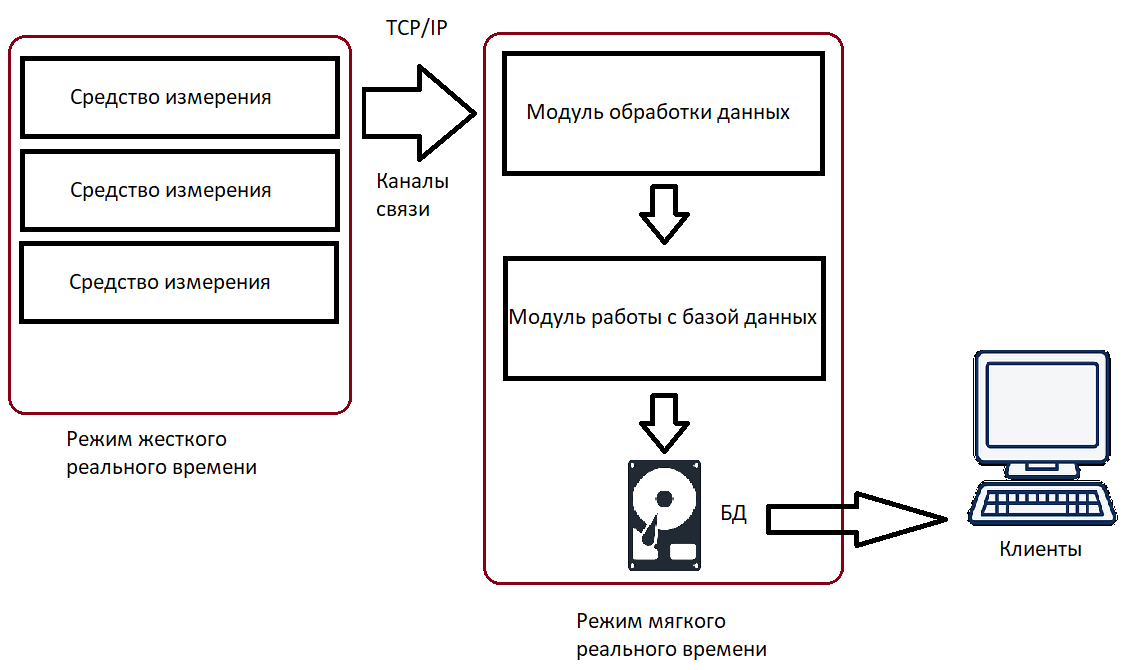
\includegraphics[width=0.95\linewidth]{image/system.png}
	\end{figure}
	На рисунке \ref{img-sys} изображена упрощенная схема системы сбора и обработки данных. Она состоит
	из двух больших блоков. Левый из них отвечает за сбор сырых данных в режиме жесткого реального времени.
	Он состоит из набора средств для измерения, способных аккумулировать сырые данные в локальную память.
	Левый блок связывается с правым модулем каналами связи, которые могут работать по протоколу TCP/IP или
	аналогичному.
	Данные из средств измерения затем отправляются в правый блок, который делает их предобработку и сохранение
	в базу данных/на диск для последующего использования и изучения подключающимися клиентами.
	\par
	В работе правого блока очень важна его пропускная способность: чем она будет выше, тем быстрее данные попадут
	в базу данных. Эта задача очень похожа на ситуацию с http-сервером, описанным ранее. Здесь так же
	присутствует множество независимых событий, а именно поступающие данные со средств измерения. 
	Потому в этой задаче можно использовать сопрограммы. А поскольку модуль работает в системе мягкого реального
	времени, то допустимо использовать для его разработки языки с управляемой средой исполнения, вроде Java и Go.
	\par
	По принципу, изображенном на рисунке \ref{img-sys}, работает система контроля износа колес
	железнодорожных составов. Во время подхода поезда к станции, средства измерения проводят все требуемые замеры
	параметров еще движущихся в тот момент колес. Затем, пока поезд стоит на остановке, сырые данные
	отправляются в модуль обработки данных, находящийся в диспетчерской, и обрабатываются. Очень важно провести
	этот анализ до отбытия поезда, чтобы можно было успеть обнаружить колеса с дефектами. Потому система
	обработки должна работать в режиме мягкого реального времени.
	\par
	На этом область применения сопрограмм не исчерпывается. Они позволяют легко организовать работу с 
	асинхронным  кодом.
	Неблокирующие операции, в том числе и асинхронный ввод--вывод, строится на обратных обработчиках (callbacks).
	Когда такого кода очень много, его становится очень трудно отлаживать и исправлять.
	Сопрограммы помогают избежать такой проблемы, представляя список обработчиков как
	последовательный кусок кода.
	
\clearpage